\documentclass[blue]{beamer}
\usetheme{Warsaw}
\setbeamertemplate{navigation
symbols}{\insertframenumber/\inserttotalframenumber}
\usepackage[francais]{babel}
\usepackage[utf8]{inputenc}
\usepackage[T1]{fontenc}
\usepackage{color}
\usepackage{listings}
\usepackage{geometry}
\usepackage{graphicx}

\definecolor{rltgrey}{rgb}{0.9,0.9,0.9}
\definecolor{rltblue}{rgb}{0.5,0.7,0.9}
%\addtobeamertemplate{footline}{\insertframenumber/\inserttotalframenumber}
\lstset{
language=SQL,                   % choose the language of the code
basicstyle=\ttfamily,           % the size of the fonts that are used for the code
numbers=left,              % where to put the line-numbers numberstyle=\footnotesize,      % the size of the fonts that are used for the line-numbers
stepnumber=0,                   % the step between two line-numbers. If it's1each line will be numbered 
numbersep=5pt,                  % how far the line-numbers are from the code
backgroundcolor=\color{rltblue},% choose the background color.
showspaces=false,               % show spaces adding particular underscores 
showstringspaces=false,         % underline spaces within strings
showtabs=false,                 % show tabs within strings adding particular underscores
frame=single,                   % adds a frame around the code
tabsize=1,                      % sets default tabsize to 2 spaces
captionpos=r,                   % sets the caption-position to bottom
breaklines=true,                % sets automatic line breaking
breakatwhitespace=false,        % sets if automatic breaks should only happen at whitespace
title=\lstname,                 % show the filename of files included with \lstinputlisting;also try caption instead of title
escapeinside={\%*}{*)},         % if you want to add a comment within your code
morekeywords={AND,ASC,avg,CHECK,COMMIT,SAVEPOINT,count,DECODE,BEGIN,DESC,DISTINCT,GROUP,IN,LIKE,NUMBER,ROLLBACK,SUBSTR,sum,VARCHAR2}        
}

\title[Système de fichiers distribué]{Système de fichiers distribué : comparaison de GlusterFS, MooseFS et Ceph avec déploiement sur la grille de calcul Grid’5000.}
\author{\it JF. Garcia, F. Lévigne, \\M. Douheret, V. Claudel}
\date{\today}
\begin{document}

%%%%%%%%%%%%%%%%%%%%%%%%%%%%%%%%%%%%%%%%%%%%%%%%%%%%%%%%%%%%%%%%%%%%%%%%%%%%%%%%%%%%%%%%%%%%%%%%
%\begin{frame}
\titlepage
%\end{frame}
%%%%%%%%%%%%%%%%%%%%%%%%%%%%%%%%%%%%%%%%%%%%%%%%%%%%%%%%%%%%%%%%%%%%%%%%%%%%%%%%%%%%%%%%%%%%%%%%
\begin{frame}{Table des Matières}
\begin{columns}[t]
\begin{column}{5cm}
\tableofcontents[sections={1-4}, hideothersubsections]
\end{column}
\begin{column}{5cm}
\tableofcontents[sections={5-8},hideothersubsections]
\end{column}
\end{columns}
%\tableofcontents[hideothersubsection]
%\tableofcontents[subsectionstyle=hide]
\end{frame}
%%%%%%%%%%%%%%%%%%%%%%%%%%%%%%%%%%%%%%%%%%%%%%%%%%%%%%%%%%%%%%%%%%%%%%%%%%%%%%%%%%%%%%%%%%%%%%%%
%%%%%%%%%%%%%%%%%%%%%%%%%%%%%%%%%%%%%%%%%%%%%%%%%%%%%%%%%%%%%%%%%%%%%%%%%%%%%%%%%%%%%%%%%%%%%%%%
%%%%%%%%%%%%%%%%%%%%%%%%%%%%%%%%%%%%%%%%%%%%%%%%%%%%%%%%%%%%%%%%%%%%%%%%%%%%%%%%%%%%%%%%%%%%%%%%
\section{Introduction}
	\subsection{Présentation du sujet}
	\begin{frame}
		\frametitle{Présentation du sujet}
		Comparaison de systèmes de fichiers distribués :
		\begin{itemize}
			\item Système de fichier (FS) : façon de stocker, organiser des informations dans un fichier
			\item Système de fichiers distribué :
			\begin{itemize}
				\item éclaté sur plusieurs serveurs % éclaté ? Un meilleur mot ?
				\item disponible depuis plusieurs clients
			\end{itemize}
		\end{itemize}
	\end{frame}

	\subsection{Le Grid'5000}
	\begin{frame}
		\frametitle{Le Grid'5000}
		\begin{itemize}
			\item Infrastructure distribué dédiée à la recherche
			\item 11 sites, dont 9 en France
			\begin{figure}
				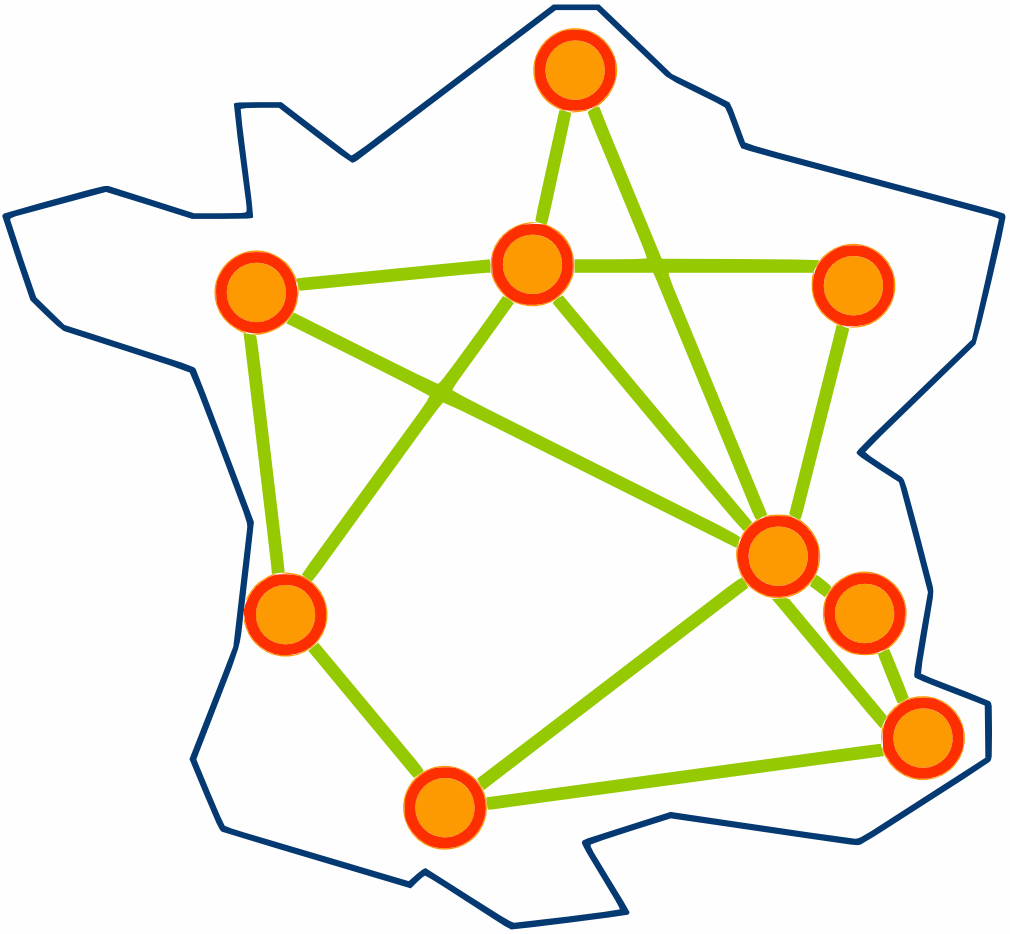
\includegraphics[width=0.3\linewidth]{../images/Site_map.png}
				\caption{Les sites français du Grid'5000}
			\end{figure}
		\end{itemize}
	\end{frame}

	\begin{frame}
		\frametitle{Travailler sur le Grid'5000}
		\begin{itemize}
			\item Connexion au \og frontend\fg~ par SSH
			\item Réservation de nœuds, pour un certain temps
			\item Déploiement d'image (OS)
		\end{itemize}

		\begin{block}{Astuce :}
			Possibilité d'effectuer une réservation à l'avance, suivit par l'exécution d'un script
		\end{block}
	\end{frame}

\section{NFS}
  \subsection{Présentation de NFS}
\begin{frame}
  \frametitle{Présentation de NFS}
  \begin{itemize}
    \item Network File System
    \item Développé par Sun Microsystem
    \item Partager des données par le réseau
    \item Méthode standard de partage entre machines Unix
  \end{itemize}
\end{frame}

\subsection{Aspect technique}
\begin{frame}
  \frametitle{Aspect technique}
  \begin{itemize}
    \item NFS et le protocole non connecté UDP
    \item Depuis la version 3, possibilité d'utiliser TCP
    \item Versions NFS définies dans différentes RFC
    \item Ensemble du protocole repensé pour NFSv4 :
    \begin{itemize}
      \item meilleur gestion de la sécurité
      \item meilleur gestion de la montée en charge
      \item système de maintenance simplifié
      \item support des protocoles TCP (par défaut) et RDMA
  \end{itemize}
  \end{itemize}
\end{frame}

\subsection{Mise en place}
	\begin{frame}
		\frametitle{Mise en place}
		\begin{itemize}
			\item Installation des paquets nfs-common et nfs-kernel-server
			\item Implémentation d'un fichier exports dans /etc
			\item Montage du partage sur les clients à l'aide de « mount »
		\end{itemize}
		\begin{block}{Pour NFSv4 :}
			Des options supplémentaires sont à définir dans /etc/exports et le type de protocole doit être spécifié lors du montage sur les clients.
		\end{block}
	\end{frame}
	
\section{GlusterFS}
	\subsection{Présentation de GlusterFS}
	\begin{frame}
		\frametitle{Présentation de GlusterFS}
		\begin{figure}
			
\includegraphics[width=0.4\linewidth]{../images/glusterfs.png}
			%\caption{Lecture de petits fichiers avec 50 serveurs}
		\end{figure}

		\begin{itemize}
			\item Licence GPLv3
			\item Se base sur FUSE (Filesystem in UserSpacE)
			\item Capacité pouvant atteindre plusieurs petabytes (1000 To)
			\item Structure simple, deux éléments logiciels : serveur et client
			\item Supporte plusieurs protocoles de communications (TCP/IP, InfiniBand)
		\end{itemize}
	\end{frame}
	
	\subsection{Mise en place}
	\begin{frame}
		\frametitle{Mise en place}
		\begin{itemize}
			\item Un serveur maitre : paquet glusterfs-server
			\item x serveurs \og normaux\fg
			\item x clients : glusterfs-client
		\end{itemize}

		\begin{block}{Note :}
			Les serveurs doivent avoir un répertoire dédié au partage
		\end{block}
	\end{frame}

	\begin{frame}
		\frametitle{Mise en place (2)}
			\begin{itemize}
				\item A partir du serveur maitre :
				\begin{itemize}
					\item Génération des fichiers de configurations (commande prévue)
					\item Envoie de fichiers aux serveurs, et aux clients
				\end{itemize}
				\item Démarrage des serveurs
				\item Montage du volume par les clients
			\end{itemize}
	\end{frame}

	\subsection{Difficultés rencontrées}
	\begin{frame}
		\frametitle{Difficultés rencontrées}
			\begin{itemize}
				\item Droit d'écriture des clients
				\item Utilisation d'InfiniBand
				\item Script de déploiement : automatisation totale
			\end{itemize}
	\end{frame}


\section{MooseFS}
\begin{frame}

\end{frame}

\section{Ceph}
        \subsection{Présentation}
        \begin{frame}
                \frametitle{Présentation de Ceph}
		\begin{itemize}
			\item Licence LGPL
			\item Créé par Sage Weill en 2007
			\item Destiné aux très grands clusters
			\item But principal : 
                              \begin{itemize}
                                      \item compatible POSIX
                                      \item complètement distribué sans point de défaillance
                              \end{itemize}
		\end{itemize}
        \end{frame}

        \subsection{Caractéristique}        
        \begin{frame}
                \frametitle{Caractéristique}
                \begin{itemize}
                        \item Caractéristiques de Ceph :
                        \begin{itemize}
                                \item robustesse
                                \item évolutivité transparente
                        \end{itemize}
                \end{itemize}
        \end{frame}

        \subsection{Fonctionnement}
        \begin{frame}
                \frametitle{Fonctionnement}
                \begin{itemize}
                        \item Trois types distincts de démons :
                        \begin{itemize}
                                \item moniteur de cluster
                                \item serveurs de métadonnées
                                \item serveurs de données
                        \end{itemize}
                \end{itemize}
        \end{frame}

        \begin{frame}
                \frametitle{Moniteur}
                \begin{itemize}
                        \item Configuration
                        \item État du cluster
                        \item Gestion des clients
                \end{itemize}
        \end{frame}

        \begin{frame}
                \frametitle{Serveurs de métadonnées}
                \begin{itemize}
                        \item Configuration
                        \item État du cluster
                        \item Gestion des clients
                \end{itemize}
        \end{frame}

\section{Comparaison}
	\subsection{Benchmark}
		\begin{frame}
		\frametitle{Benchmark}
			Actions simultanées sur plusieurs clients
			\begin{itemize}
				\item Écriture de petits fichiers
				\item Écriture de gros fichiers
				\item Lecture de petits fichiers
				\item Lecture de gros fichiers
			\end{itemize}
		\end{frame}

	\subsection{Graphiques}
		\begin{frame}
			\begin{figure}
				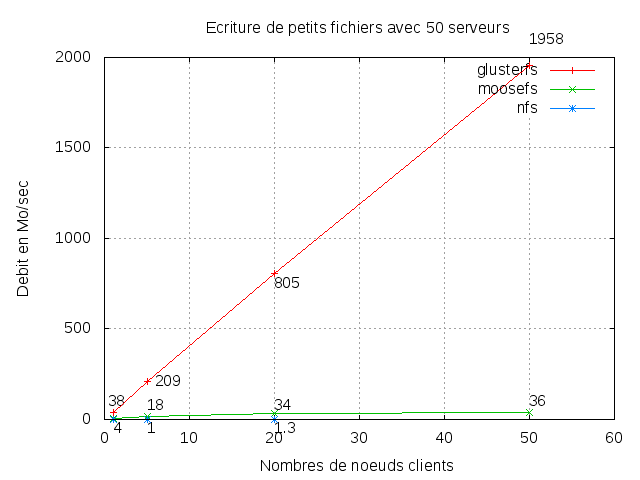
\includegraphics[width=0.75\linewidth]{../images/srv50ws2.png}
				\caption{Écriture de petits fichiers avec 50 serveurs}
			\end{figure}
		\end{frame}

		\begin{frame}
			\begin{figure}
				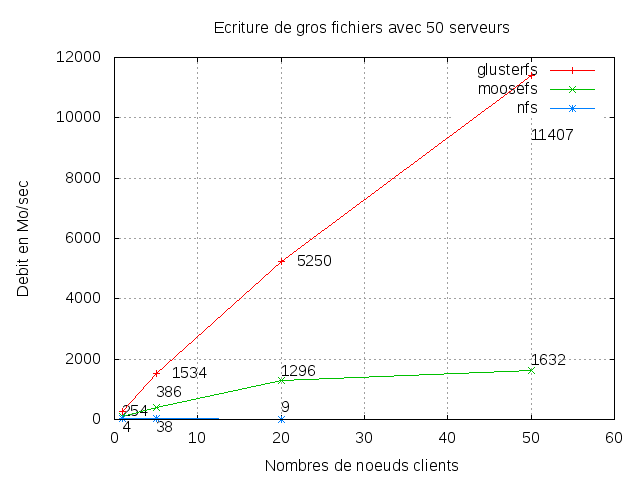
\includegraphics[width=0.75\linewidth]{../images/srv50wb2.png}
				\caption{Écriture de gros fichiers avec 50 serveurs}
			\end{figure}
		\end{frame}

		\begin{frame}
			\begin{figure}
				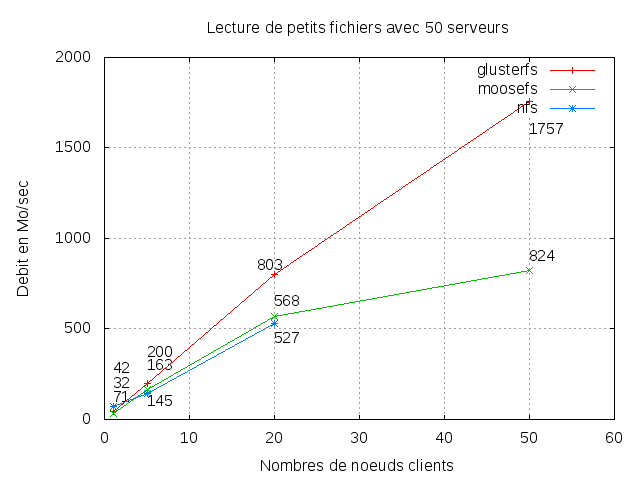
\includegraphics[width=0.75\linewidth]{../images/srv50rs2.png}
				\caption{Lecture de petits fichiers avec 50 serveurs}
			\end{figure}
		\end{frame}

		\begin{frame}
			\begin{figure}
				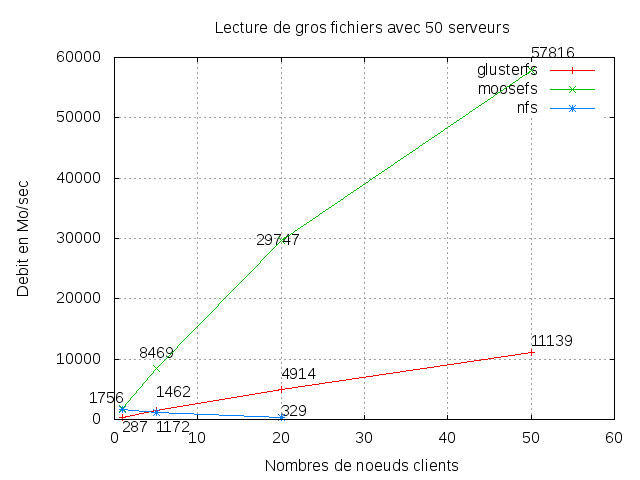
\includegraphics[width=0.75\linewidth]{../images/srv50rb2.png}
				\caption{Lecture de gros fichiers avec 50 serveurs}
			\end{figure}
		\end{frame}

	\subsection{Tableau comparatif}
		\begin{frame}
		\frametitle{Tableau comparatif}
			\begin{tabular}{|l|c|c|c|}
				\hline
				& \bf{GlusterFS} & \bf{MooseFS} & \bf{Ceph}\\
				\hline
				Facilité de mise en place & ++ & + & +\\
				\hline
				Fiabilité & ++ & ++ & -\\
				\hline
				Sécurité, disponibilité des données & + & ++ & ++ \\
				\hline
				Évolutivité & + & ++  & ++\\
				\hline
				Économe en taille disque & ++ & - & - \\
				\hline
			\end{tabular}
		\end{frame}

\section{Conclusion}
	\subsection{Difficultés rencontré}
	\begin{frame}
	\frametitle{Difficultés rencontrées}
		\begin{itemize}
			\item Prise en main du Grid'5000
			\item Partage du cluster de travail
			\item Erreurs ponctuelles lors de déploiements
		\end{itemize}
	\end{frame}

\end{document}
